\chapter{Element Parameter Groups}
\label{c:ele.groups}

Generally, element parameters are grouped into ``\vn{element} \vn{parameter} \vn{group}'' 
types. How these groups are used in a lattice element is discussed in \sref{c:ele}. 
This chapter discusses the groups in detail.

The parmeter groups are:
\begin{table}[htb]
\centering
{\tt
\begin{tabular}{llll} \toprule
 {\it Group}          & {\it Section}             & {\it Group}          & {\it Section}            \\ 
 \midrule
 ACKickerGroup        & \sref{s:ackicker.g}       & InitParticleGroup    & \sref{s:init.particle.g} \\
 AlignmentGroup       & \sref{s:alignment.g}      & LengthGroup          & \sref{s:length.g}        \\    
 ApertureGroup        & \sref{s:aperture.g}       & LordSlaveStatusGroup & \sref{s:lord.slave.g}    \\
 BMultipoleGroup      & \sref{s:bmultipole.g}     & MasterGroup          & \sref{s:master.g}        \\
 BeamBeamGroup        & \sref{s:beam.beam.g}      & OriginEleGroup       & \sref{s:origin.ele.g}    \\
 BendGroup            & \sref{s:bend.g}           & PatchGroup           & \sref{s:patch.g}         \\
 DescriptionGroup     & \sref{s:descrip.g}        & RFGroup              & \sref{s:rf.g}            \\
 DownstreamReferenceGroup & \sref{s:dreference.g} & RFAutoGroup          & \sref{s:rfauto.g}        \\
 EMultipoleGroup      & \sref{s:emultipole.g}     & ReferenceGroup       & \sref{s:reference.g}     \\
 FloorPositionGroup   & \sref{s:floor.pos.g}      & SolenoidGroup        & \sref{s:solenoid.g}      \\
 ForkGroup            & \sref{s:fork.g}           & TrackingGroup        & \sref{s:tracking.g}      \\
 GirderGroup          & \sref{s:girder.g}         & TwissGroup           & \sref{s:twiss.g}         \\
  \bottomrule
\end{tabular}
} 
\caption{Table of element parameter groups.}
\label{t:ele.param.g}
\end{table}

Element parameter groups inherit from the abstract type \vn{EleParameterGroup} which
in turn inherits from \vn{BaseEleParameterGroup}. Some
parameter groups have sub-group components. 
These sub-groups also inherit from \vn{BaseEleParameterGroup}:
\begin{example}
  abstract type BaseEleParameterGroup end
  abstract type EleParameterGroup <: BaseEleParameterGroup end
  abstract type EleParameterSubGroup <: BaseEleParameterGroup end
\end{example}

To see which element types contain a given group, use the \vn{info(::EleParameterGroup)}
method. Example:
\begin{example}
  julia> info(AlignmentGroup)
  ApertureGroup: Vacuum chamber aperture.
  ...
  Found in:
    ACKicker
    Bend
    Kicker
    ...
\end{example}

To get information on a given element parameter, including what element group the parameter is in,
use the \vn{info(::Symbol)} function using the symbol corresponding to the parameter. For example,
to get information on the multipole component \vn{Ks2L} do:
\begin{example}
  julia> info(:Ks2L)
    User name:       Ks2L
    Stored in:       BMultipoleGroup.Ks
    Parameter type:  Number
    Units:           1/m^2
    Description:     Skew, length-integrated, momentum-normalized, 
                                          magnetic multipole of order 2.
\end{example}
  
Notes:
\begin{itemize}
%
\item
All parameter groups have associated docstrings that can be accessed using the REPL help system.
%
\item
NaN denotes a real parameter that is not set.
%
\item
Parameters marked ``dependent'' are parameters calculated by \accellat and not settable by the User.
%
\item
There are several lattice element parameters that are not stored in a parameter group but are stored
alongside of the parameter groups in the element Dict. Included is the element's name, and information
on lords and slaves of the element.
%
\end{itemize}

To simplify the structure of a lattice element, certain element parameters are not stored in the 
element structure but are calculated as needed. These ``\vn{output}'' cannot be set.
See \sref{s:ele.access} for details.

%---------------------------------------------------------------------------------------------------
\section{ACKickerGroup}
\label{s:ackicker.g}

The \vn{ACKickerGroup} holds parameters associated with \vn{ACKicker} elements.

The parameters of this group are:
\begin{example}
  amp_function::Function      - Amplitude function.
\end{example}

\newpage

%---------------------------------------------------------------------------------------------------
\section{AlignmentGroup}
\label{s:alignment.g}

\begin{figure}[bt]
\centering 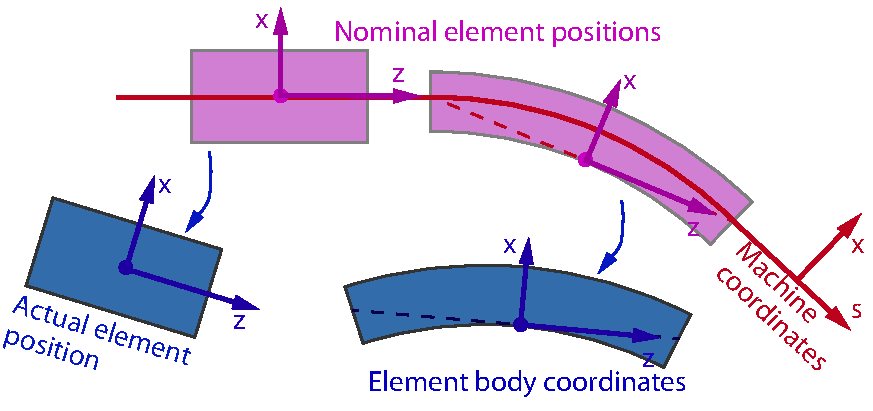
\includegraphics{alignment-ref.pdf} 
\caption[Element alignment.]  
{AlignmentGroup parameters The reference point is the origin
about which the element alignment is calculated. 
A) For straight elements, the reference point is in the center of the element. 
For \vn{Bend} elements, the reference point is at the midpoint of the chord connecting
the entrance point to the exit point. The drawing for the bend is valid for a \vn{ref_tilt}
of zero. For non-zero \vn{ref_tilt}, the outward direction from the bend center will not be
the $x$-axis. 
}  \label{f:alignment}
\end{figure}

\begin{figure}
\centering 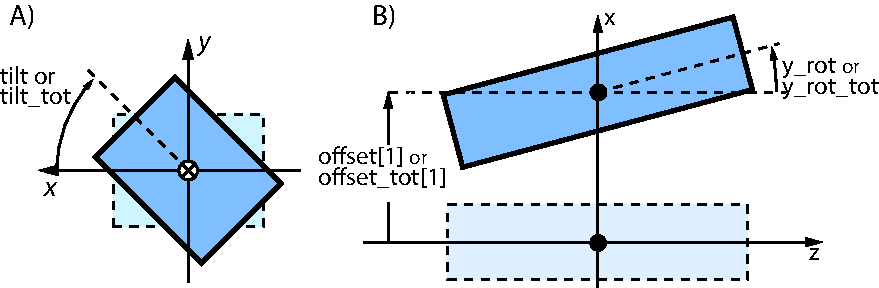
\includegraphics{alignment2.pdf} \caption[Alignment geometry.]  
{Alignment geometry. A) \vn{z_rot} (or \vn{z_rot_tot}) rotation. B) Combined
\vn{offset[1]} with \vn{y_rot} (or \vn{offset_tot[1]} with \vn{y_rot_tot}).
}  \label{f:alignment}
\end{figure}

The \vn{AlignmentGroup} gives the alignment (position and angular orientation) of the physical element 
relative to the nominal position defined by the branch coordinates (\sref{s:orient}).
Alignment is specified with respect to the ``alignment reference point'' of an element as shown
in Fig~\ref{s:alignment}. The \vn{Bend} reference point is chosen to be the center of the chord
connecting the two ends. 
This reference point was chosen over using the midpoint on the reference orbit arc since a 
common simulation problem is to simulate a bend with a \vn{z_rot} keeping the entrance and exit
endpoints fixed.

The parameters of the \vn{AlignmentGroup} are:
\begin{example}
  offset::Vector - $[x, y, z]$ offset.
  x_rot::Number  - Rotation around the x-axis.
  y_rot::Number  - Rotation around the z-axis.
  z_rot::Number  - Rotation around the z-axis. 
\end{example}
If the element is supported by a \vn{Girder}, the alignment parameters are with respect to the
orientation of the \vn{Girder} position. If there is no supporting \vn{Girder}, the alignment
parameters are with respect to the branch reference coordinates. There are output alignment
parameters:
\begin{example}
  q_align::Quaternion     - Quaternion representation of x_rot, y_rot, z_rot.
  offset_tot::Vector      - $[x, y, z]$ offset.
  x_rot_tot::Number       - Rotation around the x-axis.
  y_rot_tot::Number       - Rotation around the z-axis.
  z_rot_tot::Number       - Rotation around the z-axis. 
  q_align_tot::Quaternion - Quaternion  representation of tot rotations.
\end{example}
The ``total alignment'' parameters which have a \vn{_tot} suffix are always the alignment 
of the element with with respect to the branch coordinates.
If there is no support \vn{Girder}, the total alignment will be the same as the ``relative''
(non-tot) alignment.

The relative alignment can be set by the User. 
The total alignment is computed by \accellat based upon the relative alignment and the alignment
of any \vn{Girder}. \vn{Girder} elements themselves also have both relative and total
alignments since Girders can support other Girders.

The \vn{q_align} output parameter gives the quaternion representation of 
\vn{x_rot}, \vn{y_rot} and \vn{z_rot}. Similarly, the\vn{q_align_tot} output parameter gives the
quaternion representation of \vn{x_rot_tot}, \vn{y_rot_tot} and \vn{z_rot_tot}.

%---------------------------------------------------------------------------------------------------
\section{ApertureGroup}
\label{s:aperture.g}

\begin{figure}[bt]
\centering 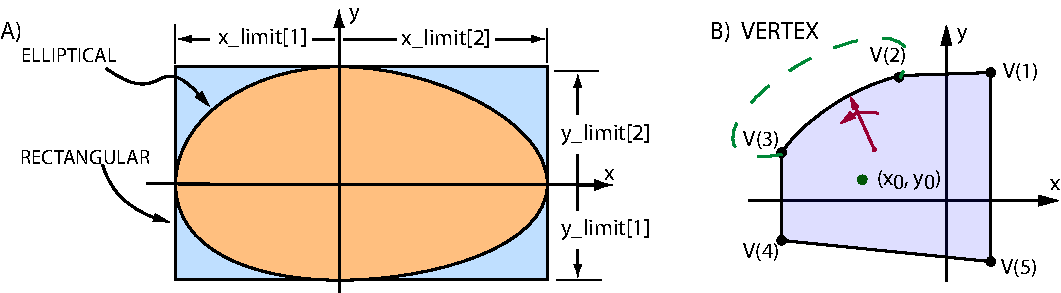
\includegraphics{apertures.pdf} \caption[Apertures.]  
{
A) RECTANGULAR and ELLIPTICAL apertures. As drawn, \vn{x_limit[1]} and \vn{y_limit[1]} are 
negative and \vn{x_limit[2]} and \vn{y_limit[2]} are positive. B) The VERTEX aperture is defined
by a set of vertices.
}  \label{f:apertures}
\end{figure}

The \vn{ApertureGroup} stores information about apertures an element may have. 
The parameters of this group are:
\begin{example}
  x_limit::Vector\{Number\}     - Min/Max x-aperture limits. (m)
  y_limit::Vector\{Number\}     - Min/Max y-aperture limits. (m)
  aperture_shape::ApertureShape - Aperture shape. Default: ELLIPTICAL
  aperture_at::BodyLoc.T        - Aperture location. Default: BodyLoc.ENTRANCE_END
  wall::Wall2D                  - Aperture defined by vertex array.
  custom_aperture::Dict         - Custom aperture information.
  aperture_shifts_with_alignment::Bool 
                                - Alignment affects aperture? Default: false.
\end{example}

The aperture location is set by the \vn{aperture_at} parameter. Possible values are
given by the \vn{BodyLoc} enum group (\sref{s:bodyloc}). The default is \vn{BodyLoc.ENTRANCE_END}.
The \vn{.EVERYWHERE} location might be problematic for some types of particle tracking and
so might not be always available.

The \vn{aperture_shape} parameter selects the shape of the aperture. Possible values are
given by the \vn{ApertureShape} Holy trait group. 
\begin{example}
  RECTANGULAR   - Rectangular shape.
  ELLIPTICAL    - Elliptical shape.
  VERTEX        - Shape defined by set of vertices.
  CUSTOM_SHAPE  - Shape defined with a custom function.
\end{example}

For \vn{RECTANGULAR} and \vn{ELLIPTICAL} shapes the \vn{x_limit} and \vn{y_limit} parameters are
used to calculate the aperture as shown in \fig{f:apertures}A. For an \vn{ELLIPTICAL} aperture,
a particle with position $(x, y)$ is outside of the aperture if any 
one of the following four conditions is true:
\begin{example}
  1) x < 0 and y < 0 and (x/x_limit[1])^2 + (y/y_limit[1])^2 > 1 
  2) x < 0 and y > 0 and (x/x_limit[1])^2 + (y/y_limit[2])^2 > 1
  3) x > 0 and y < 0 and (x/x_limit[2])^2 + (y/y_limit[1])^2 > 1
  4) x > 0 and y > 0 and (x/x_limit[2])^2 + (y/y_limit[2])^2 > 1
\end{example}
For a \vn{RECTANGULAR} aperture the corresponding four conditions are:
\begin{example}
  1) x < x_limit[1]
  2) x > x_limit[2]
  3) y < y_limit[1]
  4) y > y_limit[2]
\end{example}

Default values for the limits are \vn{-Inf} for \vn{x_limit[1]} and \vn{y_limit[1]} and 
\vn{Inf} for \vn{x_limit[2]} and \vn{y_limit[2]}.

The \vn{misalignment_moves_aperture} parameter determines whether misaligning an element 
(\sref{s:alignment.g}) affects the placement of the aperture. The default is \vn{false}. 
A common case where \vn{misalignment_moves_aperture} would be \vn{false} is when a beam pipe,
which incorporates the aperture, is not physically touching the surrounding magnet element. 
When tracking a particle, assuming that there are only apertures at the element ends, 
the order of computation with \vn{misalignment_moves_aperture} set to \vn{false} is
\begin{example}
  1) Start at upstream end of element
  2) Check upstream aperture if there is one.
  3) Convert from branch coordinates to body coordinates.
  4) Track through the element body.
  5) Convert from body coordinates to branch coordinates.
  6) Check downstream aperture if there is one.
  7) End at downstream end of element.
\end{example}
With \vn{misalignment_moves_aperture} set to \vn{true}, the computation order is 
\begin{example}
  1) Start at upstream end of element
  2) Convert from branch coordinates to body coordinates.
  3) Check upstream aperture if there is one.
  4) Track through the element body.
  5) Check downstream aperture if there is one.
  6) Convert from body coordinates to branch coordinates.
  7) End at downstream end of element.
\end{example}

The \vn{CUSTOM_SHAPE} setting for \vn{aperture_shape} indicates whether a User supplied function
is used to calculate whether the particle has hit the aperture. The function is stored
in the \vn{custom_aperture} parameter. The \vn{custom_aperture} parameter is a Dict that stores
the aperture function along with any data that the aperture calculation needs. The aperture
function must be stored in \vn{custom_aperture[:function]} and this function will be
called with the signature
\begin{example} %
  custom_aperture[:function](position::Vector, ele::Ele) -> ParticleState
\end{example}
where \vn{position} is the phase space 6-vector of the particle, \vn{ele} is the element 
with the aperture, and a \vn{ParticleState} (\sref{s:particlestate}) value is returned.

The \vn{VERTEX} setting for \vn{aperture_shape} is for defining an aperture using a 
set of vertex points as illustrated in \fig{f:apetures}B. Between vertex points, the aperture
can can follow a straight line or the arc of an ellipse. The vertex points are specified by
setting the \vn{section} parameter of \vn{ApertureGroup}. Example:
\begin{example}
  wall = Wall2D([Vertex1([1.0, 4.0]), Vertex1([-1.0, 4.0, 6.0]), 
                 Vertex1([-5.0, 1.0]), Vertex1([-5.0, -1.0]), 
                 Vertex1([1.0, -1.5)]], r0 = [-2.5, 0.5]) 
\end{example}

%---------------------------------------------------------------------------------------------------
\section{BMultipoleGroup}
\label{s:bmultipole.g}

The \vn{BMultipoleGroup} group stores magnetic multipole strengths. Also see \vn{EMultipoleGroup}.
The parameters of this group are:
\begin{example}
  vec::Vector{BMultipole1}
\end{example}
This group stores a vector of \vn{BMultipole1} structs.
The \vn{BMultipole1} structure stores the values for a magnetic multipole of a given order.
Only orders where there is a non-zero multipole are stored and there is no maximum limit to the 
order that can be stored. The multipoles will be stored in increasing order.

The \vn{BMultipole1} structure has components:
\begin{example}
  Kn::Number     - Normal normalized component. EG: "Kn2", "Kn2L".
  Ks::Number     - Skew multipole component. EG: "Ks2", "Ks2L".
  Bn::Number     - Normal field component.
  Bs::Number     - Skew field component.
  tilt::Number   - Rotation of multipole around z-axis.
  order::Int     - Multipole order.
  integrated::Union{Bool,Nothing} - Integrated multipoles or not? 
\end{example}
The \vn{order} component gives the multipole order.
There is storage for both normalized (\vn{Kn} and \vn{Ks}) and unnormalized (\vn{Bn} and \vn{Bs})
field strengths. The letter ``\vn{n}'' designates the normal component and ``\vn{s}'' designates
the skew component. 
The \accellat bookkeeping code will take care of calculating the normalized field if the unnormalized
field is set and vice versa. The reason why the structure has three components, 
normal, skew and tilt, that describe the field when only two would be sufficient is due convenience.
Having normal and skew components is convenient when magnet has multiple windings that control
both independently. A common case is combined horizontal and vertical steering magnets. On the
other hand, being able to ``misalign'' the multipole using the \vn{tilt} component is also
useful.

The dot selection operator for an element (\sref{s:ele.access}) is overloaded so that 
magnetic multipole parameters for order $J$ can be accessed using the following notation:
\hfill\break
{\tt
\begin{tabular}{lllll} \toprule
  Name        & Stored In  & Normalized & Integrated & Description \\ \midrule
  KnJ         & Kn         & Yes        & No         & Normal field. \\
  KsJ         & Ks         & Yes        & No         & Skew field. \\
  KnJL        & Kn         & Yes        & Yes        & Normal field. \\
  KsJL        & Ks         & Yes        & Yes        & Skew field. \\
  BnJ         & Bn         & No         & No         & Normal field. \\
  BsJ         & Bs         & No         & No         & Skew field. \\
  BnJL        & Bn         & No         & Yes        & Normal field. \\
  BsJL        & Bs         & No         & Yes        & Skew field. \\
  tiltJ       & tilt       & --         & --         & Field tilt. \\
  integratedJ & integrated & --         & --         & Integrated fields? \\
\bottomrule
\end{tabular}
}
\hfill\break
Substitute the multipole order for $J$ in the above table. For example, \vn{Ks2L} is the
normalized length-integrated skew field component of order 2. 

Notice that both integrated
and non-integrated fields are potentially stored in the same component of \vn{BMultipole1}.
Which type is stored is determined by the \vn{integrated} logical. If \vn{true}, the integrated
value is stored and vice versa. The \vn{integrated} setting can be different for different orders.
The setting of \vn{integrated} for a given order is determined by whether the first field component
to be set for that order is an integrated quantity or not. After the value of \vn{integrated} is set,
an error will be thrown if a something that has the opposite sense in terms of integration is 
set. For example:
\begin{example}
  @ele qq = Quadrupole(l = 0.6, Ks0L = 1.0)  # 0th order multipole is integrated
  qq.Bn1 = 0.3                  # 1st order multipole is not integrated
  qq.Ks1 = 0.5                  # This is OK.
  println(qq.integrated0)       # Will print ``true''
  println(qq.Bn0)               # Can use non-integrated component.
  qq.Bn0 = 0.7                  # Cannot set non-integrated component! error thrown!
  toggle_integrated!(qq, MAGNETIC, 0)  # toggle integrated setting for order 0.
\end{example}
In the above example, the 0th order multipole is initialized using \vn{Ks0L} so that
multipole will have the \vn{integrated} component set to \vn{true} and non-integrated values
cannot be set. However, independent of the setting of \vn{integrated}, both integrated and
non-integrated quantities can always be used in an equation. To change the value of \vn{integrated},
use the \vn{toggle_integrated!} function. This function also translates the values stored in the
field components of the structure so that the field will stay constant.

The setting of \vn{integrated} for a given multipole will also determine what stays constant
of the length of the magnet changes. If \vn{integrated} is \vn{true}, the integrated values
will be invariant and vice versa for \vn{integrated} being \vn{false}. Similarly, the setting
of the \vn{field_master} parmeter (\sref{s:master.g}) will determine whether normalized or
unnormalized quantities will stay constant if the reference energy is varied.

%---------------------------------------------------------------------------------------------------
\section{BeamBeamGroup}
\label{s:beam.beam.g}

The parameters of this group are:
\begin{example}
  n_slice::Number           - Number of slices the Strong beam is divided into.
  n_particle::Number        - Number of particle in the strong beam.
  species::Species          - Strong beam species. Default is weak particle species.
  z0_crossing::Number       - Weak particle phase space z when strong beam center
                            -   passes the BeamBeam element.
  repetition_freq:: Number  - Strong beam repetition rate.
  twiss::Twiss              - Strong beam Twiss at IP.
  sig_x::Number             - Strong beam horizontal sigma at IP.
  sig_y::Number             - Strong beam vertical sigma at IP.
  sig_z::Number             - Strong beam longitudinal sigma.
  bbi_constant::Number      - BBI constant. Set by Bmad. See manual.
\end{example}

%---------------------------------------------------------------------------------------------------
\section{BendGroup}
\label{s:bend.g}

The \vn{BendGroup} stores the parameters that characterize the shape of a \vn{Bend} element
\sref{s:bend}. The only relavent shape parameter that is not in the \vn{BendGroup} is the
length \vn{L} which is in the \vn{LengthGroup}.

The parameters of this group are:
\begin{example}
  bend_type::BendType.T     - Type of bend. Default: BendType.SECTOR.
  angle::Number             - Reference bend angle.
  g::Number                 - Reference bend strength = 1/radius.
  bend_field_ref::Number    - Reference bend field.
  L_chord::Number           - Chord length.
  tilt_ref::Number          - Reference tilt.
  e1::Number                - Entrance end pole face rotation.
  e2::Number                - Exit end pole face rotation.
  e1_rect::Number           - Entrance end pole face rotation.
  e2_rect::Number           - Exit end pole face rotation.
  edge_int1::Number         - Entrance end fringe field integral.
  edge_int2::Number         - Exit end fringe field integral
  exact_multipoles::ExactMultipoles.T  - Default: ExactMultipoles.OFF
\end{example}


Associated output parameters:
\begin{example}
  rho::Number             - Reference bend radius.
  L_sagitta::Number       - Sagitta length.
  bend_field::Number      - Actual dipole field in the plane of the bend.
  norm_bend_field::Number - Actual dipole strength in the plane of the bend.
\end{example}

\begin{figure}[ht]
{\centering 
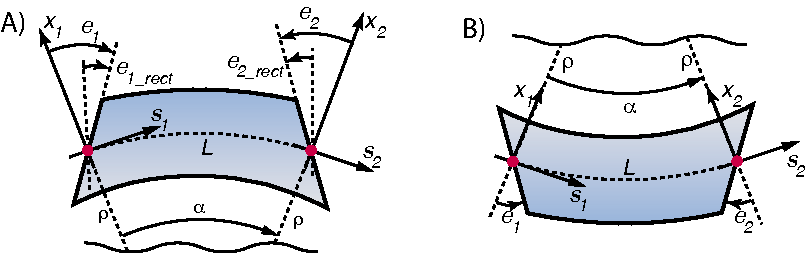
\includegraphics{bend.pdf} 
\caption[Bend geometry]{
Bend geometry. Red dots are the entry and exit points that define the origin for the
coordinate systems at the entry end $(s_1, x_1)$ and exit ends $(s_2, x_2)$ respectively. 
In the figure, the angle \vn{alpha} is denoted $\alpha$ and the radius
\vn{rho} is denoted $\rho$.
A) Bend geometry with positive bend angle. For the geometry shown, 
\vn{g}, \vn{angle}, \vn{rho}, \vn{e1}, \vn{e2}, \vn{e1_rect}, and \vn{e2_rect} are all positive.
B) Bend geometry with negative bend angle. For the geometry shown, 
\vn{g}, \vn{angle}, \vn{rho}, \vn{e1}, \vn{e2}, \vn{e1_rect}, and \vn{e2_rect} are all negative.
Note: The figures are drawn for zero \vn{ref_tilt} where the rotation axis is parallel to the 
$y$-axis. 
}
\label{f:bend}
}
\end{figure}

In detail:
  \begin{description}
  %
  \item[angle] \Newline
The total Reference bend angle. A positive \vn{angle} represents a
bend towards negative $x$ as shown in \fig{f:bend}.
  %
  \item[bend_field_ref] \Newline
The \vn{bend_field_ref} parameter is the reference magnetic bending field which is the field
that is needed for the reference particle to be bent in a circle of radius \vn{rho}
and the placement of lattice elements downstream from the bend. The actual (``total'') field is
a vector sum of
\vn{bend_field_ref} plus the value of the \vn{Bn0}  and \vn{Bs0} multipoles. If \vn{tilt0} and \vn{Bs0}
are zero, the actual field is
\begin{example}
  B-field (total) = bend_field_ref + Bn0
\end{example}
See the discussion of \vn{g} and \vn{Kn0} below for more details.
  %
  \item[bend_field (output param), norm_bend_field (output_param)] \Newline
The actual dipole bend field ignoring any skew field component which is set by \vn{Bs0}. 
The relation between this and \vn{bend_field_ref} is
\begin{example}
  bend_field = bend_field_ref + Bn0 * cos(tilt0) + Bs0 * sin(tilt0)
\end{example}
  %
  \item[bend_type] \Newline
The \vn{bend_type} parameter sets the ``logical shape'' of the bend. 
This parameter is of type \vn{BendType.T} (\sref{s:bendtype}) and can take values of
\begin{example}
  BendType.RECTANGULAR  - or
  BendType.SECTOR       - The default
\end{example}
The logical shape of a bend, in most situations, is irrelevant. 
The only case where the logical shape is used is when the bend angle is varied. 
In this case, for a \vn{SECTOR} bend, the face angles \vn{e1} and \vn{e2} are 
held constant and \vn{e1_rect} and \vn{e2_rect} are varied to keep \Eqs{eeaeea} satisfied.
  %
  \item[e1, e2] \Newline
The values of \vn{e1} and \vn{e2} gives the rotation angle of the entrance and exit pole faces
respectively with respect to the radial $x_1$ and $x_2$ axes as shown in \fig{f:bend}.
Zero \vn{e1} and \vn{e2} gives a wedge shaped magnet.
Also see \vn{e1_rect} and \vn{e2_rect}. The relationship is
\begin{equation}
  \parbox{30em} {
    e1 = e1_rect + angle/2 \\
    e2 = e2_rect + angle/2
  }
  \label{eeaeea}
\end{equation}

Note: The correspondence between \vn{e1} and \vn{e2} and the corresponding parameters used in the
SAD program \cite{Zhou:SADmaps} is:
\begin{example}
  e1(AccelLattice) =  e1(SAD) * angle + ae1(SAD)
  e2(AccelLattice) =  e2(SAD) * angle + ae2(SAD)
\end{example}
  %
  \item[e1_rect, e2_rect]
Face angle rotations like \vn{e1} and \vn{e2} except angles are measured with respect to 
fiducial lines that are parallel to each other and rotated by \vn{angle}/2 from the radial
$x_1$ and $x_2$ axes as shown in \fig{f:sbend}. 
Zero \vn{e1_rect} and \vn{e2_rect} gives a rectangular magnet shape.
  %
  \item[exact_multipoles] \Newline
The \vn{exact_multipoles} switch can be set to one of:
\begin{example}
  off                 ! Default
  vertically_pure    
  horizontally_pure  
\end{example}
This switch determines if the multipole fields, both magnetic and electric, and including the
\vn{k1} and \vn{k2} components, are corrected for the finite curvature of the reference orbit in a
bend. See \sref{s:field.exact} for a discussion of what \vn{vertically} pure versus
\vn{horizontally} pure means. Setting \vn{exact_multipoles} to \vn{vertically_pure} means that the
individual $a_n$ and $b_n$ multipole components are used with the vertically pure solutions
\begin{equation}
  \bfB = \sum_{n = 0}^\infty \left[ \frac{a_n}{n+1} \nabla \phi_n^r + \frac{b_n}{n+1} \nabla \phi_n^i \right], \qquad
  \bfE = \sum_{n = 0}^\infty \left[ \frac{a_{en}}{n+1} \nabla \phi_n^i + \frac{b_{en}}{n+1} \nabla \phi_n^r \right]
\end{equation}
and if \vn{exact_multipoles} is set to \vn{horizontally_pure} the horizontally pure solutions
$\psi_n^r$ and $\psi_n^i$ are used instead of the vertically pure solutions $\phi_n^r$ and
$\phi_n^i$.
  %
  \item[edge_int1, edge_int2] \Newline
The field integral for the entrance pole face \vn{edge_int1} is given by
\begin{equation}
  \text{edge}_1 = \int_{pole} \! \! ds \, \frac{B_y(s) \, (B_{y0} - B_y(s))}
  {2 \, B_{y0}^2}
  \label{fsbbb}
\end{equation}
For the exit pole face there is a similar equation for \vn{edge_int2}

Note: In Bmad and MAD, these integrals are represented by the product of \vn{fint} and \vn{hgap}.

Note: The SAD program uses \vn{fb1+f1} for the entrance fringe and \vn{fb2+f1} for the exit
fringe. The correspondence between the two is
\begin{example2}
  edge_int1 = (fb1 + f1) / 12
  edge_int2 = (fb2 + f1) / 12
\end{example2}

\vn{edge_int1} and \vn{edge_int2} can be related to the Enge function which is sometimes used to model the
fringe field. The Enge function is of the form
\begin{equation}
  B_y(s) = \frac{B_{y0}}{1 + \exp[P(s)]}
\end{equation}
where
\begin{equation}
  P(s) = C_0 + C_1 \, s + C_2 \, s^2 + C_3 \, s^3 + \, \ldots
\end{equation}
The $C_0$ term simply shifts where the edge of the bend is. If all the $C_n$ are zero except for
$C_0$ and $C_1$ then
\begin{equation}
  C_1 = \frac{1}{2 \, \text{field_int}}
\end{equation}
  %
  \item[g, rho (output param)] \Newline
The Reference bending radius which determines the reference coordinate system is \vn{rho} (see
\sref{s:ref}). \vn{g} = \vn{1/rho} is the ``bend strength'' and is proportional to the Reference
dipole magnetic field. \vn{g} is related to the reference magnetic field \vn{bend_field_ref} via
\begin{equation}
  \text{g} = \frac{q}{p_0} \, \text{bend_field_ref} 
  \label{gqpb}
\end{equation}
where $q$ is the charge of the reference particle and $p_0$ is the reference momentum. It is
important to keep in mind that changing \vn{g} will change the Reference orbit (\sref{s:coords.3}) and
hence will move all downstream lattice elements in space.

The total bend strength felt by a particle is the vector sum of \vn{g} plus the zeroth order
magnetic multipole. If the multipole \vn{tilt0} and \vn{Ks0} is zero, the total bend strength is
\begin{example}
  norm_bend_field = g + Kn0
\end{example}
Changing the multipole strength \vn{Kn0} or \vn{Ks0} leaves the Reference orbit and the positions of
all downstream lattice elements
unchanged but will vary a particle's orbit. One common mistake when designing lattices is to vary
\vn{g} and not \vn{Kn0} which results in downstream elements moving around. See \Sref{s:ex.chicane}
for an example.

Note: A positive \vn{g}, which will bend particles and the reference orbit in the $-x$ direction
represents a field of opposite sign as the field due a positive \vn{hkick}.
  %
  \item[h1, h2] \Newline
The attributes \vn{h1} and \vn{h2} are the curvature of the entrance and exit pole faces.
  %
  \item[L, L_arc, L_chord, L_sagitta (output param)]  \Newline
The \vn{L} parameter, which is in the \vn{LengthGroup} and not the \vn{BendGroup}, 
is the arc length of the reference trajectory through the bend.

\vn{L_chord} is the chord length from entrance point to exit point.
The \vn{L_sagitta} parameter is the sagitta length (The sagitta is the distance
from the midpoint of the arc to the midpoint of the chord). \vn{L_sagitta} can be negative and will have
the same sign as the \vn{g} parameter.
  %
  \item[L_rectangle] \Newline
The \vn{L_rectangle} parameter is the ``rectangular'' length defined to be the distance between the
entrance and exit points. The coordinate system used for the calculation is defined by the setting
of \vn{fiducial_pt}. \fig{f:rbend} shows \vn{l_rectangle} for \vn{fiducial_pt} set to
\vn{entrance_end} (the coordinate system corresponds to the entrance coordinate system of the bend).
In this case, and in the case where \vn{fiducial_pt} is set to \vn{exit_end}, the rectangular
length will be $\rho \sin\alpha$. If \vn{fiducial_pt} is set to \vn{none} or \vn{center},
\vn{l_rectangle} is the same as the chord length.
  %
  \item[ref_tilt] \Newline
The \vn{ref_tilt} attribute rotates a bend about the longitudinal axis at the entrance face of the
bend. A bend with \vn{ref_tilt} of $\pi/2$ and positive \vn{g} bends the element in the $-y$
direction (``downward''). See \fig{f:tilt.bend}. It is important to understand that \vn{ref_tilt},
unlike the \vn{tilt} attribute of other elements, bends both the reference orbit along with the
physical element. Note that the MAD \vn{tilt} attribute for bends is equivalent to the \bmad
\vn{ref_tilt}. Bends in \bmad do not have a \vn{tilt} attribute.

Important! Do not use \vn{ref_tilt} when doing misalignment studies for a machine. Trying to misalign
a dipole by setting \vn{ref_tilt} will affect the positions of all downstream elements! Rather, use the
\vn{tilt} parameter.
  \end{description}

%---------------

The attributes \vn{g}, \vn{angle}, and \vn{L} are mutually dependent. If any two are specified for
an element \accellat will calculate the appropriate value for the third.

In the local coordinate system (\sref{s:ref}), looking from ``above'' (bend viewed from positive
$y$), and with \vn{ref_tilt} = 0, a positive \vn{angle} represents a particle rotating clockwise. In
this case. \vn{g} will also be positive. For counterclockwise rotation, both \vn{angle} and \vn{g}
will be negative but the length \vn{l} is always positive. Also, looking from above, a positive
\vn{e1} represents a clockwise rotation of the entrance face and a positive \vn{e2} represents a
counterclockwise rotation of the exit face. This is true irregardless of the sign of \vn{angle} and
\vn{g}. Also it is always the case that the pole faces will be parallel when
\begin{example}
  e1 + e2 = angle
\end{example}

%---------------------------------------------------------------------------------------------------
\section{DescriptionGroup}
\label{s:descrip.g}

The components of this group are element descriptive strings:
\begin{example}
  type::String 
  ID::String 
  class::String 
\end{example}
 For example
\begin{example}
  @ele q1 = Quadrupole(type = "rotating quad", ...)
\end{example}

These strings can be used to in element searching:
\begin{example}
  eles(lat, "type = "*rot*")     # Can use these strings in searching
\end{example}
In this example \vn{lat} is the lattice that contains \vn{q1} and the \vn{eles} function
will return a vector of all elements whose \vn{type} string has the substring ``\vn{rot}''
in it.

%---------------------------------------------------------------------------------------------------
\section{DownstreamReferenceGroup}
\label{s:dreference.g}

The components of this group are:
\begin{example}
  species_ref_downstream::Species  - Reference species. 
  pc_ref_downstream::Number        - Reference momentum*c. 
  E_tot_ref_downstream::Number     - Reference total energy. 
\end{example}

Associated output parameters are:
\begin{example}
  β_ref_downstream::Number         - Reference v/c. 
  γ_ref_downstream::Number         - Reference relativistic gamma factor.
\end{example}

This group holds the reference energy and species at the downstream end of an element.
Also see the \vn{ReferenceGroup} (\sref{s:reference.g}) documentation. 
This group and \vn{ReferenceGroup} group are always paired. 
That is, these two are always both present or both not present in any given element.

For most elements, the values of the parameters in \vn{DownstreamReferenceGroup} will
be the same as the values in the corresponding \vn{ReferenceGroup} parameters.
That is, the value of \vn{species_ref_downstream} in \vn{DownstreamReferenceGroup} will be the same
as the value of \vn{species_ref} in \vn{ReferenceGroup}, the value of \vn{pc_ref_downstream} 
will be the same as \vn{pc_ref}, etc. Elements where the reference energy (here "energy" refers
to either pc_ref, E_tot_ref, β, or γ) differs between upstream and downstream
include \vn{LCavity} and \vn{Patch} elements.
Elements where the reference energy and species differ between upstream and downstream include
\vn{Foil} and \vn{Converter} elements.

Parameters of the \vn{DownstreamReferenceGroup} are not user settable and are 
calculated by the \accellat bookkeeping routines. See the \vn{ReferenceGroup} documentation
for how these parameters are calculated.

%---------------------------------------------------------------------------------------------------
\section{EMultipoleGroup}
\label{s:emultipole.g}

The \vn{EMultipoleGroup} group stores electric multipole strengths. Also see \vn{BMultipoleGroup}.
The parameters of this group are:
\begin{example}
  vec::Vector{EMultipole1}
\end{example}
This group stores a vector of \vn{EMultipole1} structs.
The \vn{EMultipole1} structure stores the values for a electric multipole of a given order.
Only orders where there is a non-zero multipole are stored and there is no maximum limit to the 
order that can be stored. The multipoles will be stored in increasing order.

The \vn{EMultipole1} structure has components:
\begin{example}
  En::Number     - Normal field component.
  Es::Number     - Skew field component.
  Etilt::Number  - Rotation of multipole around z-axis.
  order::Int     - Multipole order.
  Eintegrated::Union{Bool,Nothing} - Integrated multipoles or not? 
\end{example}
The \vn{order} component gives the multipole order.
There is storage for unnormalized (\vn{En} and \vn{Es}) field strengths however, unlike magnetic
multipoles, there are no components for normalized field strengths. 
The letter ``\vn{n}'' designates the normal component and ``\vn{s}'' designates the skew component. 
There is also a \vn{Etilt} component which will tilt the entire multipole \sref{???}.
The reason why the structure has three components, 
normal, skew and tilt, that describe the field when only two would be sufficient is due convenience.
Having normal and skew components is convenient when magnet has multiple windings that control
both independently.

The dot selection operator for an element (\sref{s:ele.access}) is overloaded so that 
electric multipole parameters for order $J$ can be accessed using the following notation:
\hfill\break
{\tt
\begin{tabular}{lllll} \toprule
  Name         & Stored In   & Integrated & Description \\ \midrule
  EnJ          & En          & No         & Normal field. \\
  EsJ          & Es          & No         & Skew field. \\
  EnJL         & En          & Yes        & Normal field. \\
  EsJL         & Es          & Yes        & Skew field. \\
  EtiltJ       & Etilt       & --         & Field tilt. \\
  EintegratedJ & Eintegrated & --         & Integrated fields? \\
  \bottomrule
\end{tabular}
} 
\hfill\break
Substitute the multipole order for $J$ in the above table. For example, \vn{Es2L} is the
normalized length-integrated skew field component of order 2. 

Notice that both integrated
and non-integrated fields are potentially stored in the same component of \vn{EMultipole1}.
Which type is stored is determined by the \vn{Eintegrated} logical. If \vn{true}, the integrated
value is stored and vice versa. The \vn{Eintegrated} setting can be different for different orders.
The setting of \vn{Eintegrated} for a given order is determined by whether the first field component
to be set for that order is an integrated quantity or not. After the value of \vn{Eintegrated} is set,
an error will be thrown if a something that has the opposite sense in terms of integration is 
set. For example:
\begin{example}
  @ele qq = Quadrupole(l = 0.6, Es0L = 1.0)  # 0th order is integrated
  qq.En1 = 0.3                  # 1st order multipole is not integrated
  qq.Es1 = 0.5                  # This is OK.
  println(qq.Eintegrated0)      # Will print ``true''
  println(qq.En0)               # Can use non-integrated component.
  toggle_integrated!(qq, ELECTRIC, 0)  # change integrated setting for order 0.
\end{example}
In the above example, the 0th order multipole is initialized using \vn{Es0L} so that
multipole will have the \vn{Eintegrated} component set to \vn{true} and non-integrated values
cannot be set. However, independent of the setting of \vn{Eintegrated}, both integrated and
non-integrated quantities can always be used in an equation. To change the value of \vn{Eintegrated},
use the \vn{toggle_integrated!} function. This function also translates the values stored in the
field components of the structure so that the field will stay constant.

The setting of \vn{Eintegrated} for a given multipole will also determine what stays constant
of the length of the magnet changes. If \vn{Eintegrated} is \vn{true}, the integrated values
will be invariant with length changes and vice versa if \vn{integrated} is \vn{false}. 
Similarly, the setting of the \vn{field_master} parmeter (\sref{s:master.g}) will determine 
whether normalized or unnormalized quantities will stay constant if the reference energy is varied.

%---------------------------------------------------------------------------------------------------
\section{FloorPositionGroup}
\label{s:floor.pos.g}

The \vn{FloorPositionGroup} stores position and orientation information in the Floor coordinate 
system. The components of this group are:
\begin{example}
  r_floor::Vector          - [x,y,z] position. 
  q_floor::Quat            - Quaternion orientation. 
\end{example}

%---------------------------------------------------------------------------------------------------
\section{ForkGroup}
\label{s:fork.g}

The components of this group are:
\begin{example}
  to_line::Union{BeamLine, Nothing}   - Beam line to fork to
  to_ele::String                      - Element forked to.
  direction::Int                      - Longitudinal Direction of injected beam.
  new_branch::Bool                    - New or existing `to_line`?
\end{example}

This group is used with a \vn{Fork} element and specifies how the fork element attaches to
another branch.

%---------------------------------------------------------------------------------------------------
\section{GirderGroup}
\label{s:girder.g}

The components of this group are:
\begin{example}
  supported::Vector{Ele}    - Elements supported by girder. 
\end{example}


%---------------------------------------------------------------------------------------------------
\section{InitParticleGroup}
\label{s:init.particle.g}

The components of this group are:
\begin{example}
  orbit::Vector{Number}     - Phase space 6-vector. 
  spin::Vector{Number}      - Spin 3-vector. \end{example}

%---------------------------------------------------------------------------------------------------
\section{LengthGroup}
\label{s:length.g}

The components of this group are:
\begin{example}
  L::Number               - Length of element. 
  s::Number               - Starting s-position. 
  s_downstream::Number    - Ending s-position. 
  orientation::Int        - Longitudinal orientation. +1 or -1. 
\end{example}

%---------------------------------------------------------------------------------------------------
\section{LordSlaveStatusGroup}
\label{s:lord.slave.g}
\label{s:lord.enum}
\label{s:slave.enum}

The components of this group are: \\
\begin{example}
  lord_status::Lord.T     - Lord status. 
  slave_status::Slave.T   - Slave status. 
\end{example}

The possible values of \vn{lord_status} are:
\vspace*{-0.4ex} \\
\begin{tabular}{ll}
  Lord & \\
  \indnt .NOT       & -- Not a lord \\
  \indnt .SUPER     & -- Is a Super lord (\sref{c:super}) \\
  \indnt .MULTIPASS & -- Is a Multipass lord (\sref{c:multipass}) \\
\end{tabular}
\hfill \break \vskip -1.2ex

The possible values of \vn{lord_status} are: \\
\vspace*{-0.4ex} \\
\begin{tabular}{ll}
  Slave & \\
  \indnt .NOT       & -- Not a slave \\
  \indnt .SUPER     & -- Is a Super slave (\sref{c:super}) \\
  \indnt .MULTIPASS & -- Multipass slave (\sref{c:multipass}) \\
\end{tabular}
\hfill \break \vskip -1.2ex

Notice that elements that are supported by a \vn{Girder} are not marked as slaves to the \vn{Girder}
although the supported elements will have a pointer to the supporting girder.

This group is used in lattice element lord/slave bookkeeping (\sref{c:lord.slave.book}). See this
section for more details.

%---------------------------------------------------------------------------------------------------
\section{MasterGroup}
\label{s:master.g}

The components of this group are:
\begin{example}
  is_on::Bool = true
  field_master::Bool = false         # Does field or normalized field stay constant with energy changes?
\end{example}

%---------------------------------------------------------------------------------------------------
\section{OriginEleGroup}
\label{s:origin.ele.g}

The components of this group are:
\begin{example}
  origin_ele::Ele           - Origin reference element. Default is NULL_ELE.
  origin_ele_ref_pt::Loc.T  - Origin reference point. Default is Loc.CENTER. 
\end{example}

The \vn{OriginEleGroup} is used with \vn{Fiducial}, \vn{FloorShift}, and \vn{Girder} elements.
The \vn{OriginEleGroup} is used to set the coordinate reference frame from which 
the orientation set by the \vn{AlignmentGroup} is measured. To specify that the floor coordinates are
to be used, set the \vn{origin_ele} to \vn{NULL_ELE}. Typically this is the same as using the
beginning element of the first branch of a lattice as long as the first element does not have
any orientation shifts.


%---------------------------------------------------------------------------------------------------
\section{PatchGroup}
\label{s:patch.g}

\begin{figure}[tb]
  \centering
  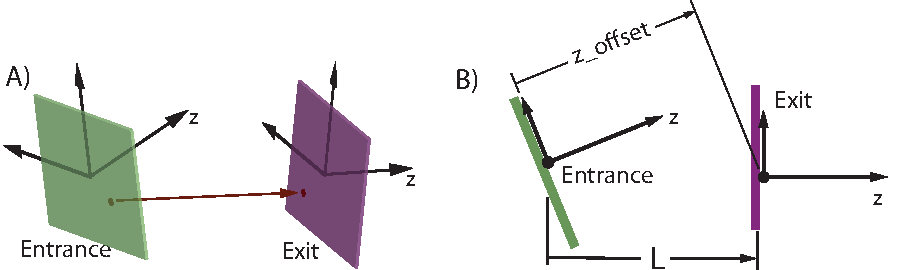
\includegraphics[width=5in]{patch.pdf}
  \caption[Patch Element.]
{A) A \vn{patch} element can align its exit face arbitrarily with respect to its entrance face. The
red arrow illustrates a possible particle trajectory form entrance face to exit face. B) The
reference length of a \vn{patch} element, if \vn{ref_coords} is set to the default value of
\vn{exit_end}, is the longitudinal distance from the entrance origin to the exit origin using the
reference coordinates at the exit end as shown. If \vn{ref_coords} is set to \vn{entrance_end}, the
length of the patch will be equal to the \vn{z_offset}.}
  \label{f:patch}
\end{figure}

The components of this group are:
\begin{example}
  t_offset::Number          - Time offset. 
  E_tot_offset::Number      - Total energy offset. Default is NaN (not used). 
  E_tot_exit::Number        - Fix total energy at exit end. Default is NaN (not used). 
  pc_exit::Number           - Reference momentum*c at exit end. Default is NaN (not used). 
  flexible::Bool            - Flexible patch? Default is false. 
  L_user::Number            - User set Length? Default is NaN (length calculated by bookkeeping code). 
  ref_coords::BodyLoc.T     - Reference coordinate system used inside the patch. Default is BodyLoc.EXIT_END.
\end{example}

A straight line element like a \vn{drift} or a \vn{quadrupole} has the exit face parallel to the
entrance face. With a \vn{patch} element, the entrance and exit faces can be arbitrarily oriented
with respect to one another as shown in \fig{f:patch}A.

\index{rigid patch}\index{inflexible patch}
\index{flexible patch}
There are two different ways the orientation of the exit face is determined. Which way is used is
determined by the setting of the \vn{flexible} attribute.  With the \vn{flexible} attribute set to
\vn{False}, the default, The exit face of the \vn{patch} will be determined from the offset, tilt
and pitch attributes as described in \sref{s:patch.coords}. This type of \vn{patch} is called
``rigid'' or ``inflexible'' since the geometry of the \vn{patch} is solely determined by the
\vn{patch}'s attributes as set in the lattice file and is independent of everything else. Example:
\begin{example}
  pt: patch, z_offset = 3.2   ! Equivalent to a drift
\end{example}

With \vn{flexible} set to \vn{True}, the exit face is taken to be the reference frame of the
entrance face of the next element in the lattice. In this case, it must be possible to compute the
reference coordinates of the next element before the reference coordinates of the \vn{patch} are
computed. A \vn{flexible} \vn{patch} will have its offsets, pitches, and tilt as dependent
parameters (\sref{s:depend}) and these parameters will be computed appropriately. Here the
\vn{patch} is called ``flexible'' since the geometry of the patch will depend upon the geometry of
the rest of the lattice and, therefore, if the geometry of the rest of the lattice is modified (is
``flexed''), the geometry of the \vn{patch} will vary as well. See Section~\sref{s:ex.erl} for an
example.

The coordinates of the lattice element downstream of a \vn{flexible} \vn{patch} can be computed
if there is a \vn{fiducial} element (\sref{s:fiducial}) somewhere downstream or if there is a
\vn{multipass_slave} (\sref{c:multipass}) element which is just downstream of the \vn{patch} or at
most separated by zero length elements from the \vn{patch}. In this latter case, the
\vn{multipass_slave} must represent an $N$\Th pass slave with $N$ greater than 1. This works since
the first pass slave will be upstream of the \vn{patch} and so the first pass slave will have its
coordinates already computed and the position of the downstream slave will be taken to be the same
as the first pass slave. Notice that, without the \vn{patch}, the position of multipass slave
elements are independent of each other.

With \vn{bmad_standard} tracking (\sref{s:tkm}) A particle, starting at the upstream face of the
\vn{patch}, is propagated in a straight line to the downstream face and the suitable coordinate
transformation is made to translate the particle's coordinates from the upstream coordinate frame to
the downstream coordinate frame (\sref{s:patch.std}). In this case the \vn{patch} element can be
thought of as a generalized \vn{drift} element.

If there are magnetic or electric fields within the \vn{patch}, the tracking method through the
\vn{patch} must be set to either \vn{runge_kutta} or \vn{custom}. Example:
\begin{example}
  pa2: patch, tracking_method = runge_kutta, field_calc = custom, 
              mat6_calc_method = tracking, ...
\end{example}
In order to supply a custom field when \vn{runge_kutta} tracking is used, \vn{field_calc}
(\sref{s:integ}) needs to be set to \vn{custom}. In this case, custom code must be supplied for
calculating the fields as a function of position (\sref{s:custom.ele}).

The \vn{E_tot_offset} attribute offsets the
reference energy:
\begin{example}
  E_tot_ref(exit) = E_tot_ref(entrance) + E_tot_offset (eV)
\end{example}
Setting the \vn{E_tot_offset} attribute will affect a particle's $p_x$, $p_y$ and $p_z$ coordinates
via \Eqs{ppp} and \eq{ppppp}.  Notice that \vn{E_tot_offset} does not affect a particle's actual
energy, it just affects the difference between the particle energy and the reference energy.

Alternatively, to set the reference energy, the \vn{E_tot_set} or \vn{p0c_set} attributes can be
used to set the reference energy/momentum at the exit end. It is is an error if more than one of
\vn{E_tot_offset}, \vn{E_tot_set} and \vn{p0c_set} is nonzero.

\vn{Important}: \bmad may apply the energy transformation either before or after the coordinate
transformation. This matters when the speed of the reference particle is less than $c$. For this
reason, and due to complications involving PTC, it is recommended to use two patches in a row when
both the orbit and energy are to be patched.

A \vn{patch} element can have an associated electric or magnetic field (\sref{s:fieldmap}). This can
happen, for example, if a patch is used at the end of an injection line to match the reference
coordinates of the injection line to the line being injected into (\sref{s:ex.inj}) and the patch
element is within the field generated by an element in the line being injected into. In such a case,
it can be convenient to set what the reference coordinates are since the orientation of any fields
that are defined for a patch element will be oriented with respect to the patch element's reference
coordinates. For this, the \vn{ref_coords}
parameter of a patch can be used. Possible settings are:
\vn{ref_coords} are:
\begin{example}
  entrance_end  !
  exit_end      ! Default
\end{example}
The default setting of \vn{ref_coords} is \vn{exit_end} and with this the reference coordinates are
set by the exit end coordinate system (see \fig{f:patch}). If \vn{ref_coords} is set to
\vn{entrance_end}, the reference coordinates are set by the entrance end coordinate system. Example:
\begin{example}
  p1: patch, x_offset = 1, x_pitch = 0.4   ! L = 0.289418 see below
  p2: p1, ref_coords = entrance_end        ! L = 0
\end{example}
Here \vn{p1} has \vn{ref_coords} set to \vn{exit_end} (the default). \vn{p2} inherits the parameters
of \vn{p1} and sets \vn{ref_coords} to \vn{entrance_end}.

It is important to keep in mind that if there are multiple patches in a row, while two different
configurations may be the same in a geometrical sense the total length may not be the same. For
example:
\begin{example}
  pA: patch, x_offset = 1    ! L = 0
  pB: patch, x_pitch = 0.4   ! L = 0
  sum: line = (pA, pB)
\end{example}
The configuration of \vn{pA} followed by \vn{pB} is equivalent geometrically to the \vn{p1} patch
above but the total length of the \vn{(pA, pB)} line is zero which is different from the length of
\vn{p1}.

Unfortunately, there is no intuitive way to define the ``\vn{length}'' \vn{L} of a patch. This is
important since the transit time of the reference particle is the element length divided by the
reference velocity. And the reference transit time will affect how the phase space $z$ coordinate
changes through the patch via \Eq{zbctt}. If the parameter \vn{user_sets_length} is set to True, the
value of \vn{l} set in the lattice file will be used (default is zero). \vn{user_sets_length} is set
to False (the default), the length of a patch is calculated depending upon the setting of
\vn{ref_coords}.  If \vn{ref_coords} is set to \vn{exit_end}, the length of the patch is calculated
as the perpendicular distance between the origin of the patch's entrance coordinate system and the
exit face of the patch as shown in \fig{f:patch}B. If \vn{ref_coords} is set to \vn{entrance_end},
the length is calculated as the perpendicular distance between the entrance face and the origin of
the exit coordinate system. In this case, the length will be equal to \vn{z_offset}.

To provide flexibility, the \vn{t_offset} attribute can be
used to offset the reference time. The reference time at the exit end of the patch
\vn{t_ref(exit)} is related to the reference time at the beginning of the patch \vn{t_ref(entrance)}
via
\begin{example}
  t_ref(exit) = t_ref(entrance) + t_offset + dt_travel_ref
\end{example}
where \vn{dt_travel_ref} is the time for the reference particle to travel through the patch.
\vn{dt_travel_ref} is defined to be:
\begin{example}
  dt_travel_ref = L / beta_ref
\end{example}
Where \vn{L} is the length of the \vn{patch} and \vn{beta_ref} is the reference velocity/c at the
exit end of the element. That is, the reference energy offset is applied {\em before} the reference
particle is tracked through the patch. Since this point can be confusing, it is recommended that a
\vn{patch} element be split into two consecutive patches if the \vn{patch} has finite \vn{l} and
\vn{E_tot_offset} values.

While a finite \vn{t_offset} will affect the reference time at the end of a patch, a finite
\vn{t_offset} will {\em not} affect the time that is calculated for a particle to reach the end of
the patch. On the other hand, a finite \vn{t_offset} will affect a particle's $z$ coordinate via
\Eqs{zbctt}. The change in $z$, $\delta z$ will be
\begin{equation}
  \delta z = \beta \cdot c \cdot \text{t_offset}
\end{equation}
where $\beta$ is the normalized particle speed (which is independent of any energy patch). Another
way of looking at this is to note that In a drift, if the particle is on-axis and on-energy, t and
t_ref change but z does not change. In a time patch (a patch with only \vn{t_offset} finite), t_ref
and z change but t does not.

When a lattice branch contains both normally oriented and reversed elements
(\sref{s:ref.construct}), a \vn{patch}, or series of \vn{patches}, which reflects the $z$ direction
must be placed in between. Such a \vn{patch}, (or patches) is called a \vn{reflection} \vn{patch}.
See Section~\sref{s:reflect.patch} for more details on how a reflection patch is defined. In order
to avoid some confusing conceptual problems involving the coordinate system through a reflection
patch, Runge-Kutta type tracking is prohibited with a reflection patch.\footnote
  {
In general, Runge-Kutta type tracking through a patch is a waste of time unless electric or magnetic
fields are present.
  }

\index{wall}
Since the geometry of a \vn{patch} element is complicated, interpolation of the chamber wall in the
region of a patch follows special rules. See section~\sref{s:wall.vacuum} for more details.



%---------------------------------------------------------------------------------------------------
\section{RFGroup}
\label{s:rf.g}

The components of this group are:
\begin{example}
  frequency::Number         - RF frequency. 
  harmon::Number            - RF frequency harmonic number. 
  voltage::Number           - RF voltage. 
  gradient::Number          - RF gradient. 
  phase::Number             - RF phase. 
  multipass_phase::Number   - RF Phase added to multipass elements. 
  cavity_type::Cavity.T     - Cavity type. Default is Cavity.STANDING_WAVE. 
  n_cell::Int               - Number of cavity cells. Default is 1. 
\end{example}


Whether \vn{voltage} or \vn{gradient} is kept constant with length changes is determined by
the setting of \vn{field_master} (\sref{s:master.g}). If \vn{field_master} is \vn{true}, the
\vn{gradient} is kept constant and vice versa.

%---------------------------------------------------------------------------------------------------
\section{RFAutoGroup}
\label{s:rfauto.g}

The components of this group are:
\begin{example}
  do_auto_amp::Bool           - Will autoscaling set auto_amp? Default is true. 
  do_auto_phase::Bool         - Will autoscaling set auto_phase? Default is true. 
  auto_amp::Number            - Auto RF field amplitude scale value. 
  auto_phase::Number          - Auto RF phase value. 
\end{example}

%---------------------------------------------------------------------------------------------------
\section{ReferenceGroup}
\label{s:reference.g}

The components of this group are:
\begin{example}
  species_ref::Species          - Reference species entering end. 
  pc_ref::Number                - Reference momentum*c upstream end. 
  E_tot_ref::Number             - Reference total energy upstream end. 
  time_ref::Number              - Reference time upstream end. 
  time_ref_downstream::Number   - Reference time downstream end. 
  extra_dtime_ref::Number       - User set reference time change.
  dE_ref::Number                - Sets change in reference energy.
\end{example}

Associated output parameters are:
\begin{example}
  β_ref::Number                 - Reference v/c upstream end. 
  γ_ref::Number                 - Reference relativistic gamma factor.
\end{example}

This group holds the reference energy, species, and time parameters at the upstream 
end of a lattice element.
Also see the \vn{DownstreamReferenceGroup} group documentation (\sref{s:dreference.g}).
The \vn{DownstreamReferenceGroup} group holds the reference energy and species
at the downstream end of the element. 
This group and \vn{DownstreamReferenceGroup} group are always paired. 
That is, these two are always both present or both not present in any given element.

For a \vn{Beginning} element, parameters of this group are user settable except for the 
\vn{dvoltage_ref} parameter. For all other element types, except for \vn{dvoltage_ref} and
\vn{extra_dtime_ref}, the parameters of this
group are calculated by the \accellat bookkeeping routines and are not user settable. 

For most elements, the values of the parameters in \vn{DownstreamReferenceGroup} will
be the same as the values in the corresponding \vn{ReferenceGroup} parameters.
That is, the value of \vn{species_ref_downstream} in \vn{DownstreamReferenceGroup} will be the same
as the value of \vn{species_ref} in \vn{ReferenceGroup}, the value of \vn{pc_ref_downstream} 
will be the same as \vn{pc_ref}, etc. Elements where the reference energy (here "energy" refers
to either pc_ref, E_tot_ref, β, or γ) differs between upstream and downstream are elements with
a non-zero \vn{dvoltage_ref} and include \vn{LCavity} and \vn{Patch} elements.
Elements where the reference energy and species differ between upstream and downstream include
\vn{Foil} and \vn{Converter} elements.

For elements where \vn{dvoltage_ref} is nonzero the downstream reference energy 
\vn{E_tot_ref_downstream} is calculated from the upstream \vn{E_tot_ref} via the equation
\begin{example}
  E_tot_ref_downstream = E_tot_ref + dvoltage_ref * |Q_ref|
\end{example}
where \vn{|Q_ref|} is the magnitude of the charge of the reference particle in units of the
fundamental charge. Once \vn{E_tot_ref_downstream} has been calculated, the downstream values
of pc, β, and γ are calculated using the standard formulas. Notice that \vn{dvoltage_ref} is 
completely independent from the actual voltage seen by a particle which is set by the \vn{voltage}
parameter of the \vn{RFGroup}.

The downstream reference time \vn{time_ref_downstream} is calculated via
\begin{example}
  time_ref_downstream = time_ref + transit_time + extra_dtime_ref
\end{example}
where \vn{transit_time} is the time to transit the element assuming a straight line trajectory
and a linear energy change throughout the element. . The general formula
for the transit time is
\begin{example}
  transit_time = L * (E_tot_ref + E_tot_ref_downstream) / (c * (pc_ref + pc_ref_downstream))
\end{example}
where \vn{L} is the length of the element and \vn{c} is the speed of light.
For elements where there is no energy
change (\vn{dvoltage_ref} = 0), the transit time calculation simplifies to
\begin{example}
  transit_time = L / (β_ref * c)
\end{example}

The \vn{extra_dtime_ref} parameter in the above is ment as a correction to take into account 
for particle motion that is not straight or acceleration that is not linear in energy. For example,
in a wiggler, \vn{extra_dtime_ref} can be used to correct for the oscillatory nature of the
particle trajectories. 
Since \accellat does not do tracking (see the discussion in \sref{c:design}), \vn{extra_dtime_ref}
must be calculated by the User.


%---------------------------------------------------------------------------------------------------
\section{SolenoidGroup}
\label{s:solenoid.g}

The components of this group are:
\begin{example}
  Ksol::Number        - Normalized solenoid strength.       
  Bsol::Number        - Solenoid field. 
\end{example}

%---------------------------------------------------------------------------------------------------
\section{TrackingGroup}
\label{s:tracking.g}

The components of this group are:
\begin{example}
  num_steps::Int    - Number of steps. 
  ds_step::Number   - Step length. 
\end{example}

%---------------------------------------------------------------------------------------------------
\section{TwissGroup}
\label{s:twiss.g}

In development

The components of this group are:
\begin{example}
\end{example}
